% !TEX root = ../rapport.tex
\chapter{Simulations et r\'esultats}\label{simu}

\section{Outils de programmation}
Nos contraintes d'implémentation lors de ce TER étaient d'utiliser le simulateur de réseaux \href{http://wsnet.gforge.inria.fr/}{WSNET}. Ce simulateur (décrit comme un "simulateur évènementiel pour les grands réseaux de capteurs sans fils") est constitué d'un ensemble de modules en langage $C$. Ces modules correspondent aux différentes couches réseaux (voir figure \ref{structWSNET}).
\begin{figure}[h]
\centering
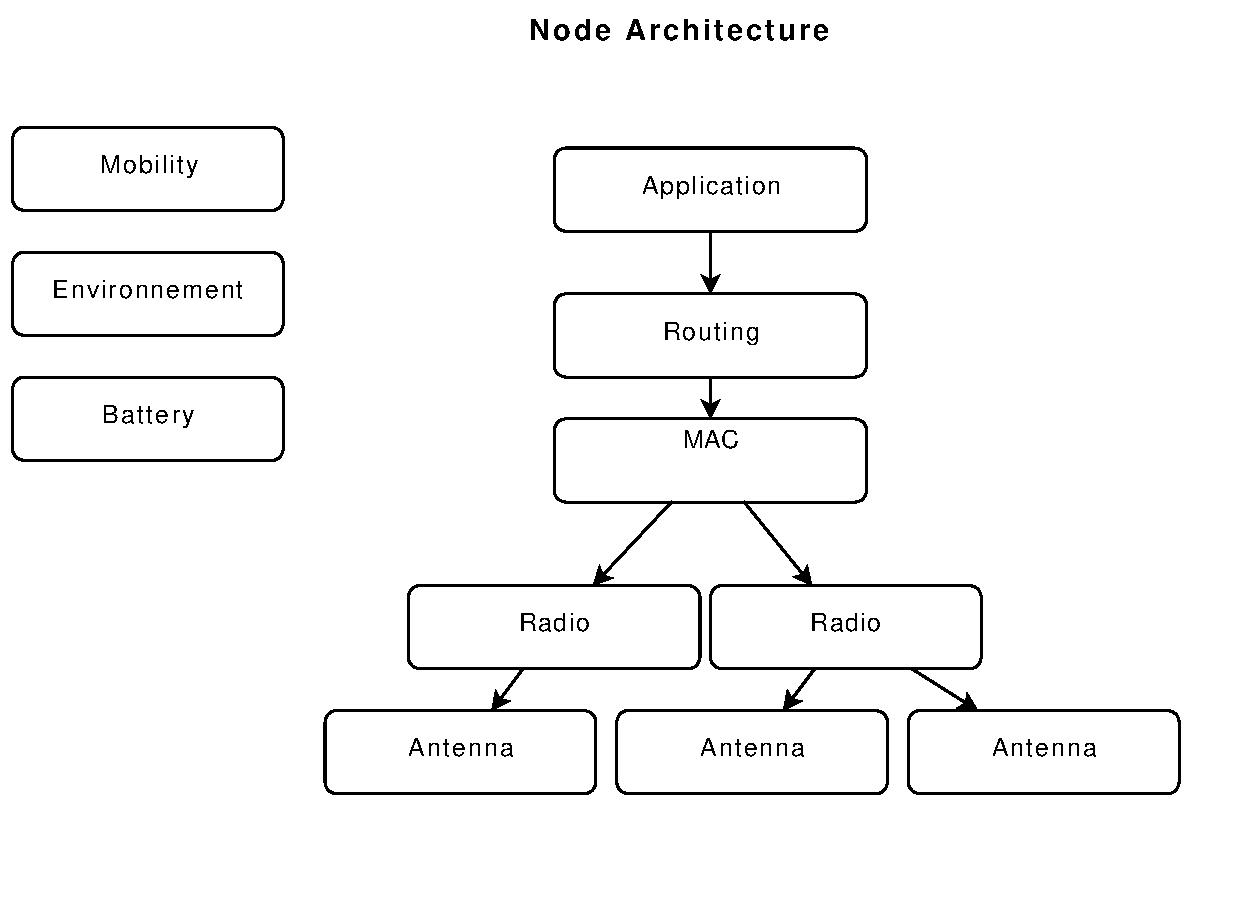
\includegraphics[scale=0.5]{Simus/WSNET.pdf}
\caption{Architecture de WSNET}
\label{structWSNET}
\end{figure}
Cette bibliothèque est développée par trois chercheurs lyonnais : Guillaume Chelius, (chercheur INRIA), Antoine Fraboulet (maitre de conférence) et Elyes Ben Hamida (doctorat).

Dans le cadre de notre TER, nous avons développé onze modules supplémentaires pour WSNET : 
\begin{itemize}
	\item un module utilitaire contenant des structures de données
	\item un module gérant la consommation énergétique
	\item un module gérant la couche liaison (protocole mac) sans interférences mais qui appelle le module de consommation d'énergie
	\item sept modules de routage (le cœur de notre TER)
		\begin{itemize}
			\item uni-cast : Flow Augmentation \cite{Chang2000}
			\item diffusion aveugle
			\item RBOP \cite{Cartigny2005}
			\item LBOP \cite{Cartigny2005}
			\item BIP \cite{Wieselthier2000}
			\item LBIP \cite{Ingelrest2008}
			\item DLBIP \cite{Champ2009DLBIP}
		\end{itemize}
	\item un module gérant la couche application et permettant la diffusion depuis plusieurs sources
\end{itemize}
~\\
Nous avons également écrit différents scripts $bash$ et $C++$ afin d'automatiser les phases de tests ainsi que la collecte des résultats. Enfin, nous avons développé un visualisateur de graphes sous \href{http://qt.nokia.com/}{Qt} afin de pouvoir vérifier la pertinence de nos résultats sur une topologie donnée.


\section{Paramètres de simulation}

À l'aide de tous ces outils, nous avons pu nous lancer dans les simulations des différents algorithmes de routage. Pour cela, nous avons fixé différents paramètres :

\renewcommand\arraystretch{1.6}
\begin{tabular}{| l | c |}
\hline
nombre de capteurs (nœuds du graphe) & $100$ \\ \hline
rayon d'émission maximum & $30m$ \\ \hline
taille de la zone où sont répartis les capteurs & $1000 \times 1000 m^2$ \\ \hline
durée de simulation & $10000s$ \\ \hline
temps entre deux diffusions & $2s$ \\ \hline
\end{tabular}

Ces paramètres sont communs à toutes nos simulations. Cependant, certains autres paramètres varient : la topologie du réseau, les constantes $\alpha$ et $c$ du modèle énergétique et la quantité d'énergie initiale des nœuds.


\section{Topologie aléatoire}
Ces phases de test ont été effectuées en utilisant un générateur de graphes aléatoires connexes que nous avons écrit en C++. Cette topologie permet de se rapprocher au mieux du contexte général des réseaux de capteurs.

Le modèle énergétique que nous avons choisi d'utiliser fixe la consommation énergétique lors de l'envoi d'information à $ r^\alpha + c $. Nous avons lancé deux phases de tests avec des valeurs différentes pour les constantes $\alpha$ et $c$.

\subsection{Modèle énergétique simple}
Le modèle énergétique le plus simple (mais aussi le plus éloigné de la réalité) utilise les valeurs suivantes pour les constantes énergétiques : $\alpha = 2$ et $c = 0$.

\subsubsection{Time To First Fall et PerCent Node}


\begin{figure}[H]
\begin{bigcenter}
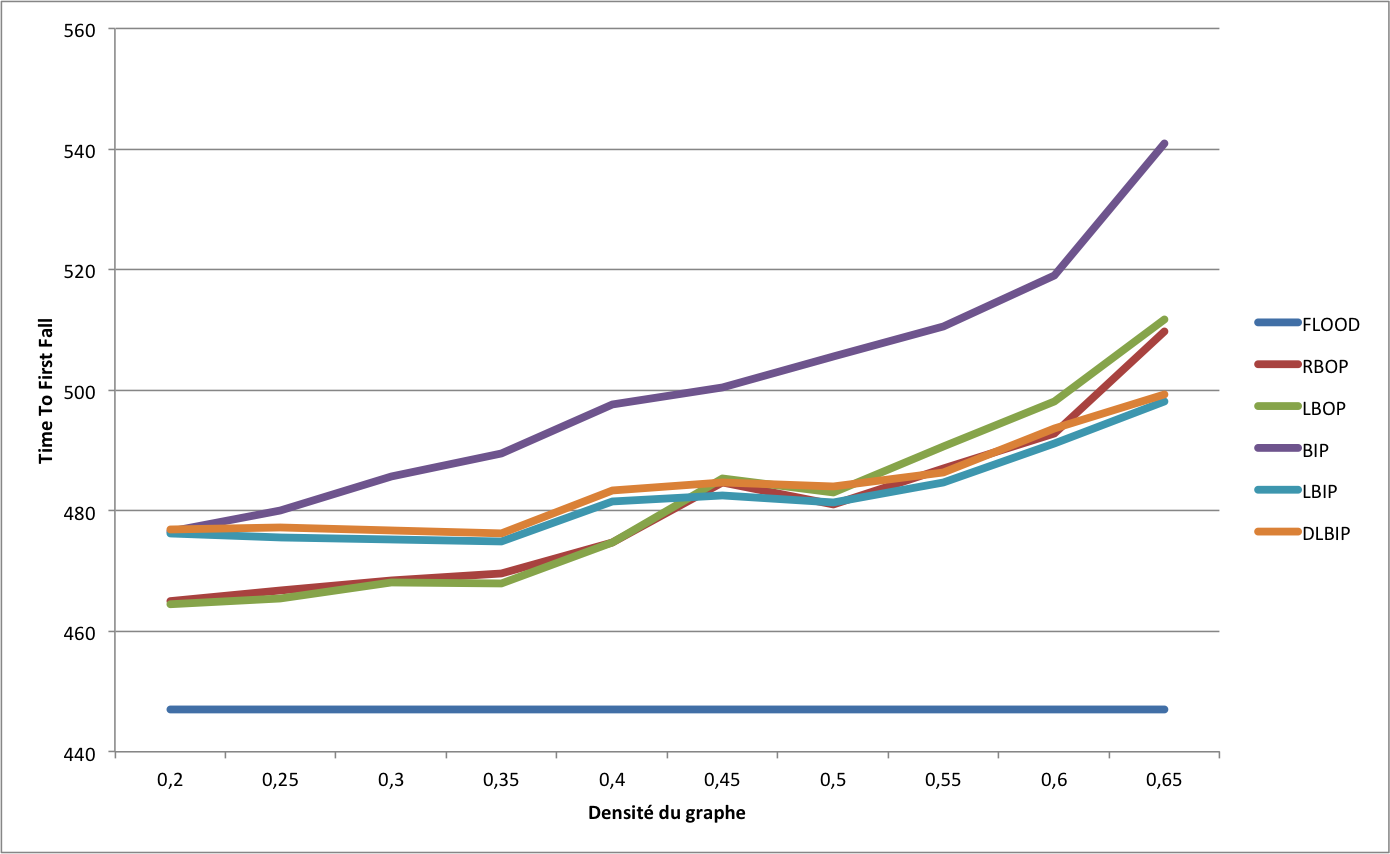
\includegraphics[scale=0.75]{Simus/ttff_2_0}
\caption{TTFF, pour $\alpha = 2$ et $c = 0$}
\label{TTFF1}
\end{bigcenter}
\end{figure}

La figure \ref{TTFF1} représente le temps avant qu'un premier noeud soit à court d'énergie pour pouvoir envoyer un message. Ce temps ne dépends pas de la densité pour la diffusion aveugle (FLOOD) puisque ce protocole présente le même comportement quelque que soit le réseau.

Le fait que BIP offre les meilleures durées de vie pour les 2 définitions (figure \ref{TTFF1} et figure \ref{PCN1}) confirme les estimations théoriques que cet algorithme est à ce jour parmi ceux approximant le mieux la solution optimale \cite{Liang2002}. Ainsi pour le TTFF, nous constatons que pour une densité comprise entre 0.2 et 0.45, DLBIP est  entre 1\% et 13\% moins performant que BIP puis LBOP entre 0.45
et 0.65, TTFF(LBOP) représente 90\% de TTFF(BIP). Cependant lorsque l'on considère la deuxième définition (figure \ref{PCN1} et figure \ref{PCN1bis}) , nous constatons la nette supériorité de BIP. Cette définition est plus représentative de la réalité car elle 
considère non plus le temps avant la mort d'un seul noeud mais de 25\% des noeuds du réseau. De plus, parmi les algorithmes locaux, DLBIP a la plus grande durée de vie.  


\begin{figure}[H]
\begin{bigcenter}
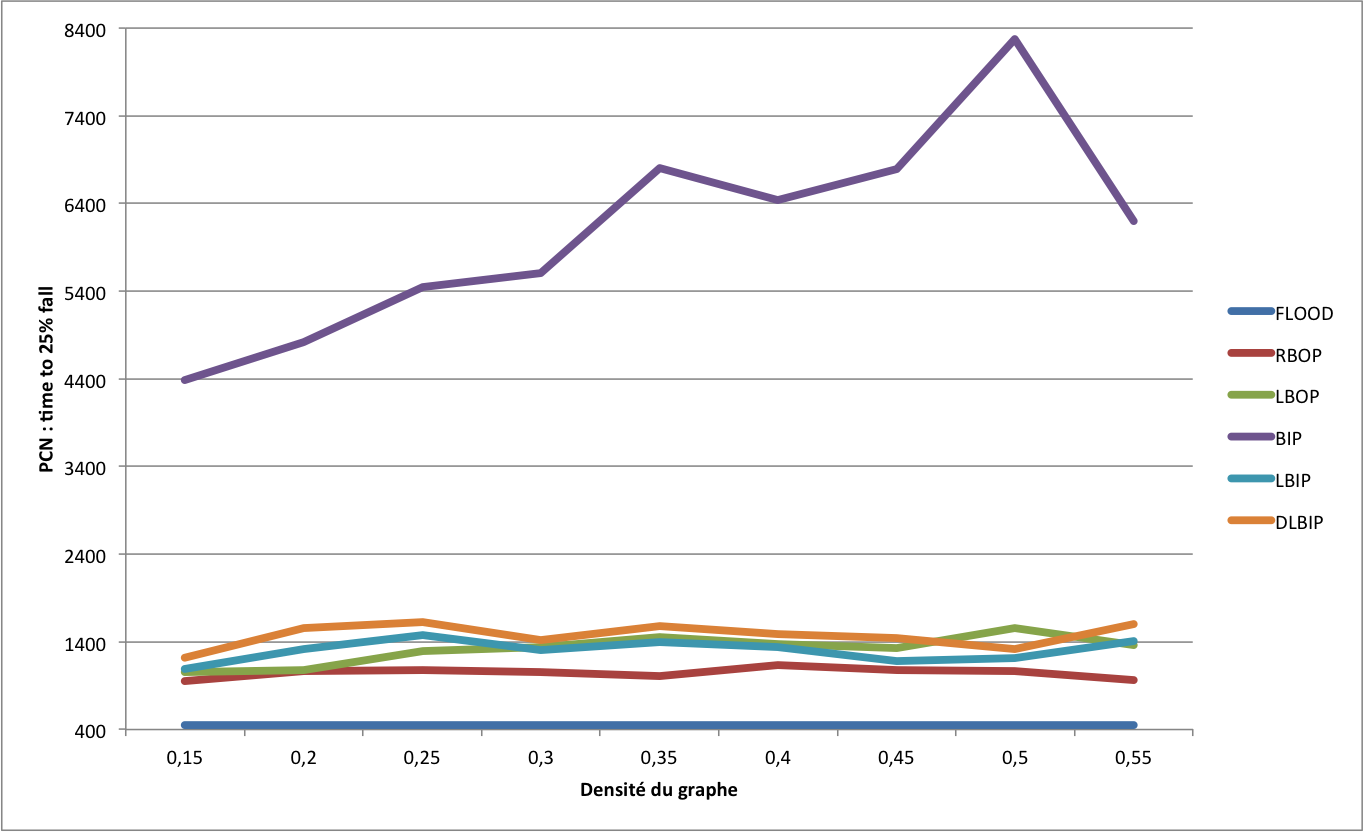
\includegraphics[scale=0.75]{Simus/pcn_2_0}
\caption{Percent Node, pour $\alpha = 2$ et $c = 0$ }
\label{PCN1}
\end{bigcenter}
\end{figure}

\begin{figure}[H]
\begin{bigcenter}
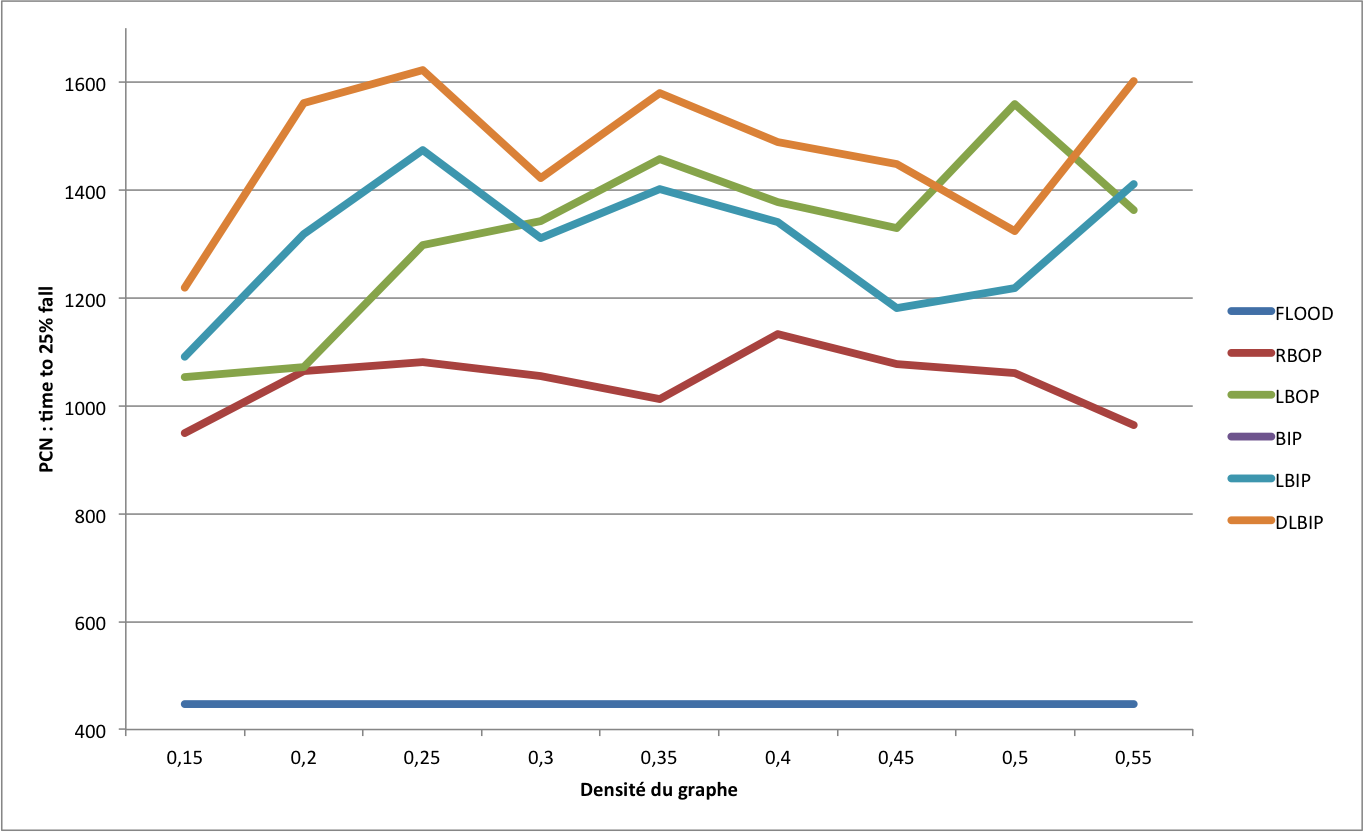
\includegraphics[scale=0.75]{Simus/pcn_2_0_zoom}
\caption{Percent Node: zoom}
\label{PCN1bis}
\end{bigcenter}
\end{figure}


\subsubsection{Lose Connectivity}

La connectivité du réseau est difficile à préserver. Prévoir le comportement d'un protocole vis à vis de cette propriété est un problème où il reste beaucoup à faire comme en témoigne la figure \ref{LC1}. Les résultats de nos simulations
concernant la perte de connectivité montrent que cette grandeur varie fortement en fonction de la densité et de la topologie du réseau. 

\begin{figure}[H]
\begin{bigcenter}
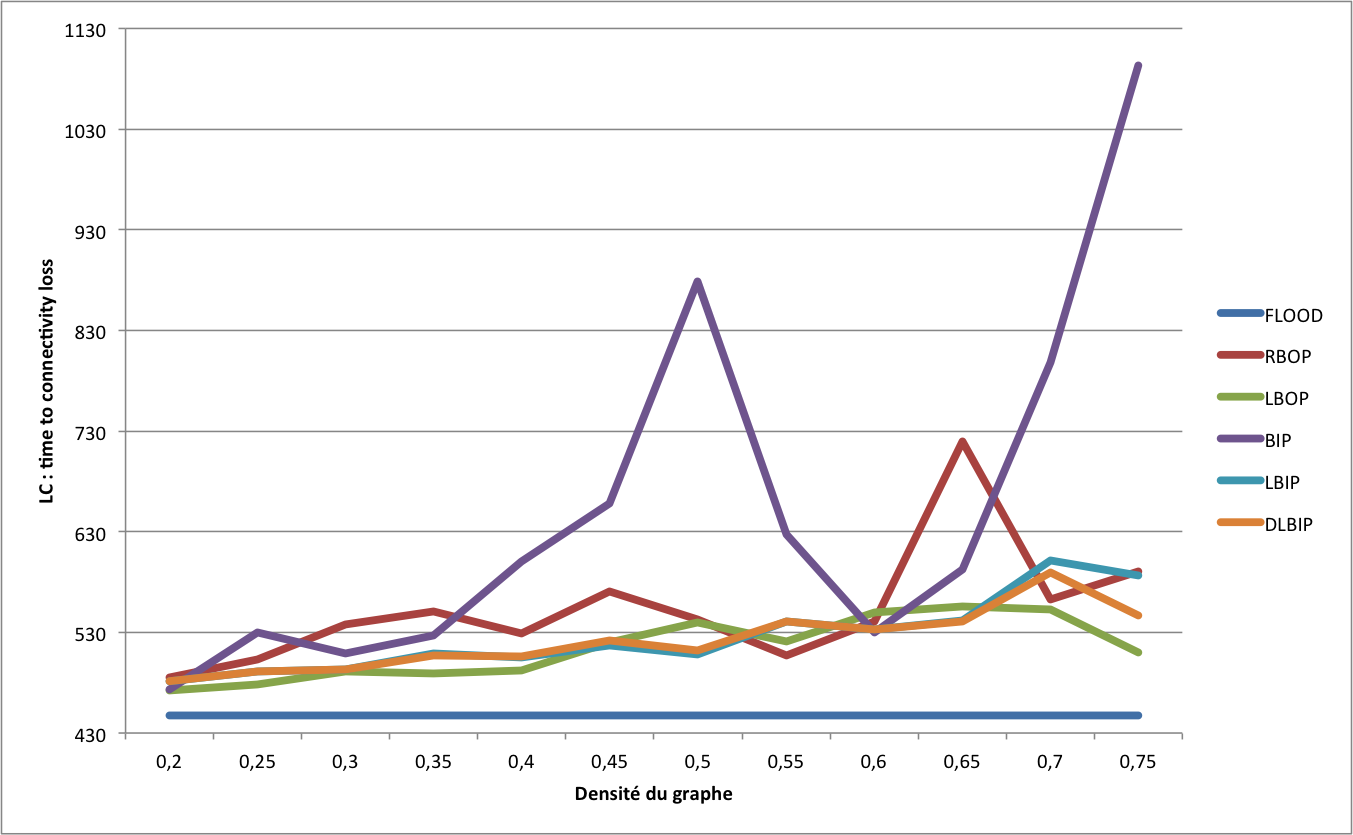
\includegraphics[scale=0.75]{Simus/lc_2_0}
\caption{Perte de connectivité, pour $\alpha = 2$ et $c = 0$}
\label{LC1}
\end{bigcenter}
\end{figure}



\subsection{Modèle énergétique plus réaliste}
Ce modèle énergétique un peu plus réaliste utilise les valeurs suivantes pour les constantes énergétiques : $\alpha = 4$ et $c = 10^6$ \cite{Rodoplu1998}.


\subsubsection{Time To First Fall et PerCent Node }
Lorsqu'il s'agit du TTFF, le changement des constantes $\alpha$ et $c$ inverse les résultats: la figure \ref{TTFF2} montre que DLBIP et LBIP présentent de moins bonnes caractéristiques que LBOP et RBOP. Cependant pour la deuxième définition qui 
traduit le temps écoulé jusqu'à la perte de 25\% des noeuds, la figure \ref{PC2} met en évidence la similarité des résultats avec ceux obtenus pour $\alpha = 2$ et $c = 0$: DLBIP reste le meilleur.
\begin{figure}[H]
\begin{bigcenter}
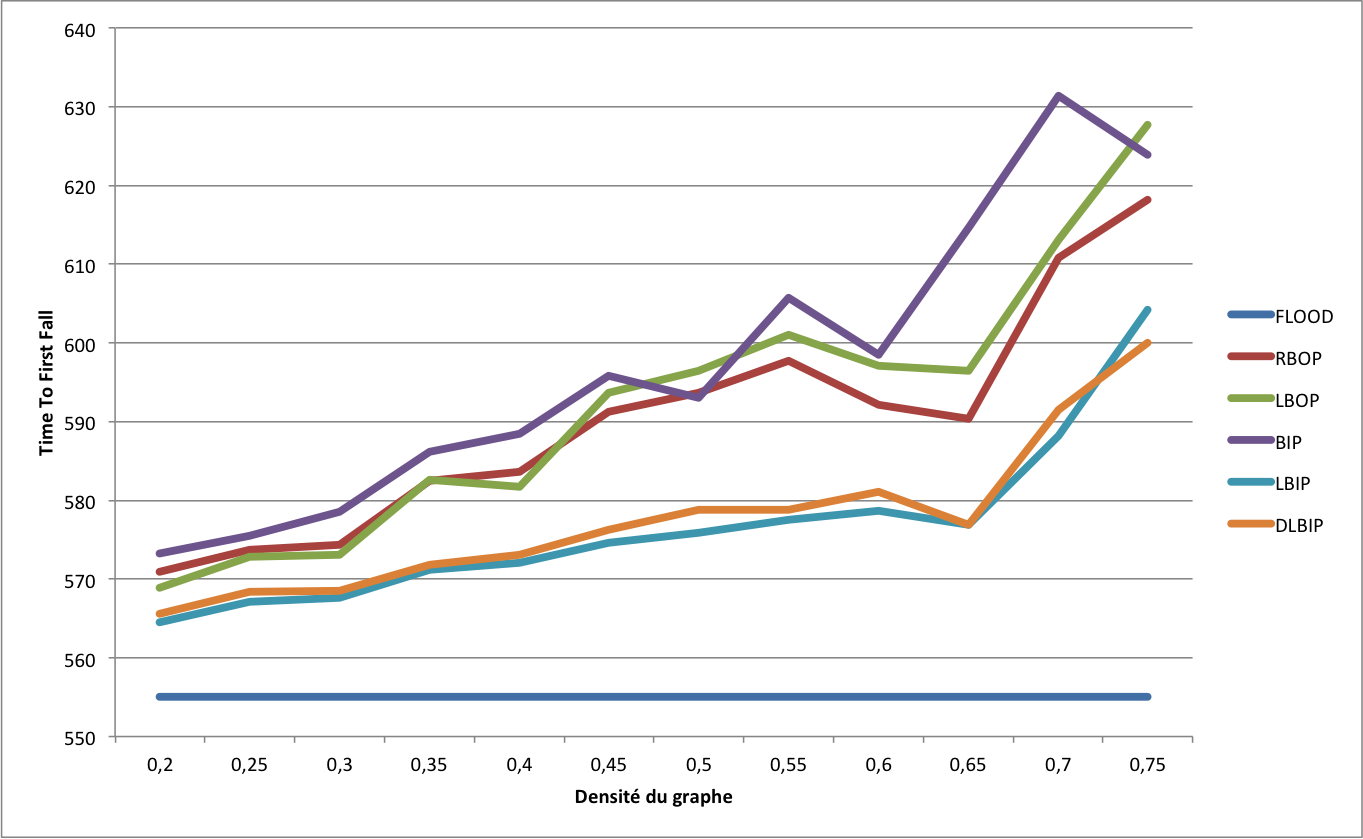
\includegraphics[scale=0.75]{Simus/ttff_4_10p6}
\caption{TTFF, pour $\alpha = 4$ et $c = 10^6$. }
\label{TTFF2}
\end{bigcenter}

\begin{bigcenter}
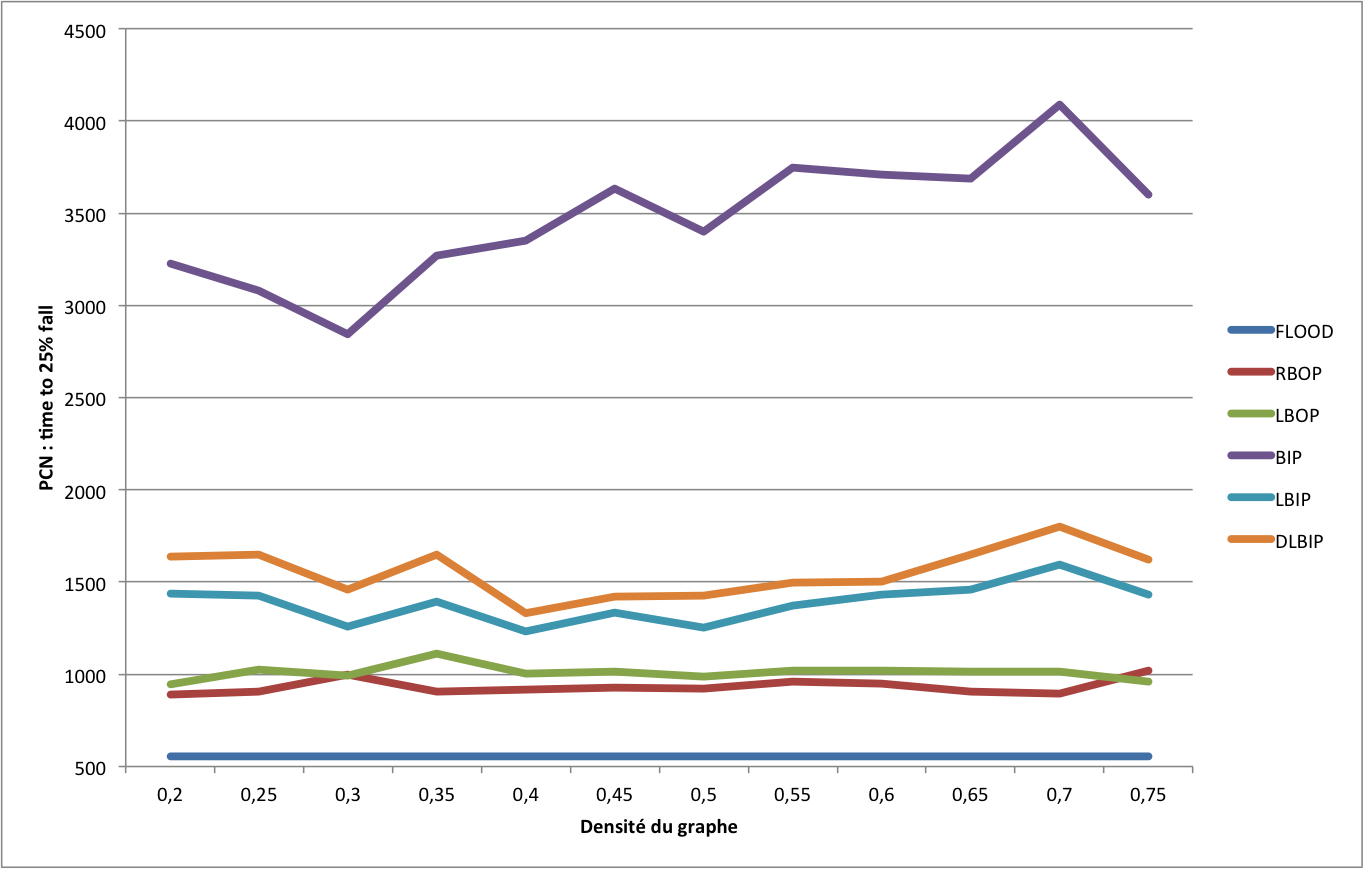
\includegraphics[scale=0.75]{Simus/pcn_4_10p6}
\caption{Percent Node, pour $\alpha = 4$ et $c = 10^6$.}
\label{PC2}
\end{bigcenter}
\end{figure}


\subsubsection{Lose Connectivity}

Avec pour modèle énergétique $\alpha = 4$ et $c = 10^6$, la figure \ref{LC2} souligne de nouveau que la perte de connectivité fluctue de façon brutale. Cependant BIP préserve dans l'ensemble mieux la connectivité du réseau.


\begin{figure}[H]
\begin{bigcenter}
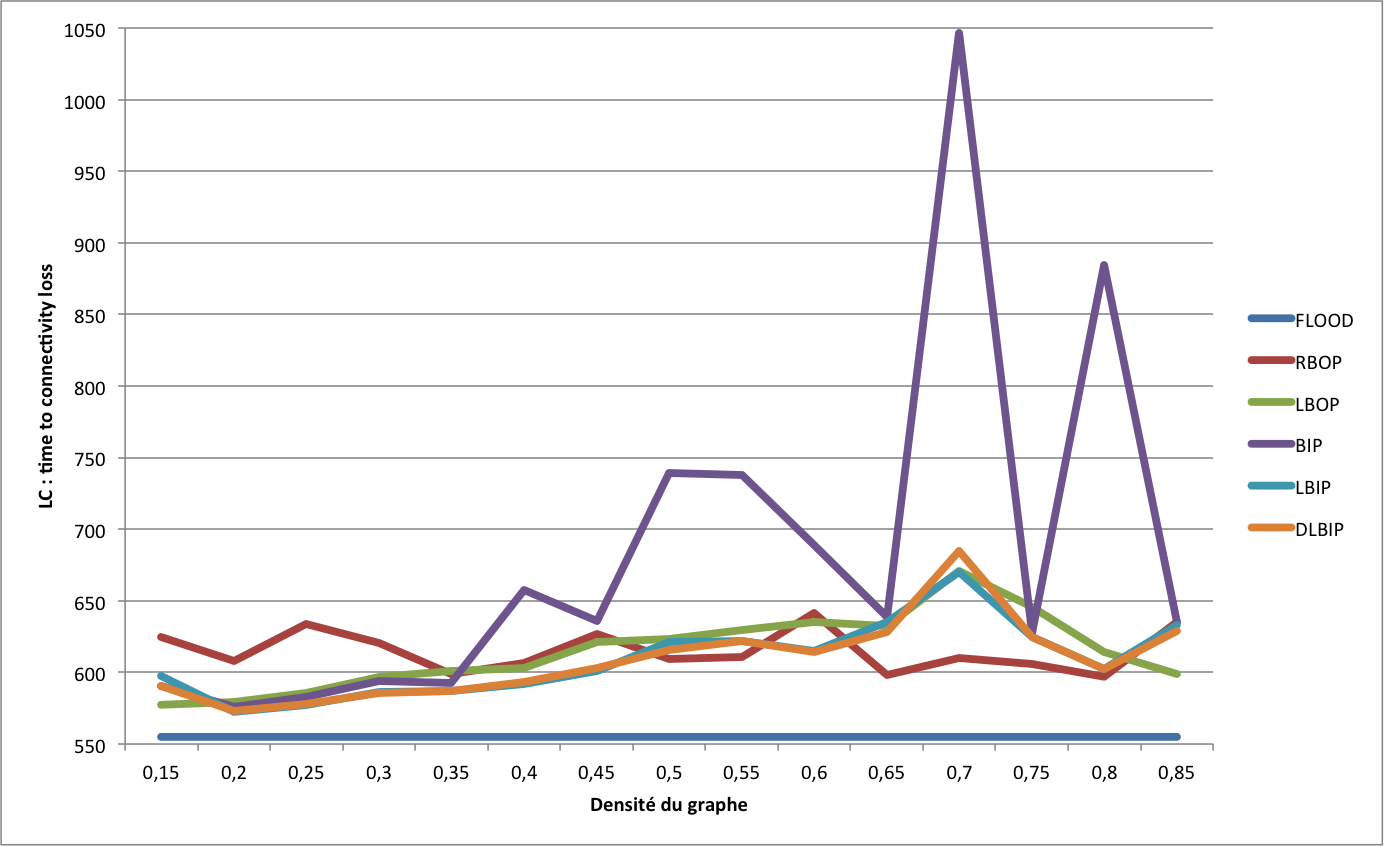
\includegraphics[scale=0.75]{Simus/lc_4_10p6}
\caption{Perte de connectivité, pour $\alpha = 4$ et $c = 10^6$.}
\label{LC2}
\end{bigcenter}
\end{figure}